\documentclass[12pt,letterpaper]{article}
\usepackage{fullpage}
\usepackage[top=2cm, bottom=4.5cm, left=2.5cm, right=2.5cm]{geometry}
\usepackage{amsmath,amsthm,amsfonts,amssymb,amscd}
\usepackage{lastpage}
\usepackage{enumerate}
\usepackage{fancyhdr}
\usepackage{mathrsfs}
\usepackage[table,xcdraw]{xcolor}
\usepackage{graphicx}
\usepackage{listings}
\usepackage{hyperref}

\hypersetup{%
  colorlinks=true,
  linkcolor=blue,
  linkbordercolor={0 0 1}
}
 
\renewcommand\lstlistingname{Algorithm}
\renewcommand\lstlistlistingname{Algorithms}
\def\lstlistingautorefname{Alg.}

\lstdefinestyle{Python}{
    language        = Python,
    frame           = lines, 
    basicstyle      = \footnotesize,
    keywordstyle    = \color{blue},
    stringstyle     = \color{green},
    commentstyle    = \color{red}\ttfamily
}

\setlength{\parindent}{0.0in}
\setlength{\parskip}{0.05in}

% Edit these as appropriate
\newcommand\course{CSE 3500}
\newcommand\hwnumber{5}                   % <-- homework number
\newcommand\release{October 20, 2022}     % <-- release date
\newcommand\due{November 3, 2022}        % <-- homework number

\pagestyle{fancyplain}
\headheight 35pt
\lhead{\course}
\chead{\textbf{\Large Homework \hwnumber}}
\rhead{Released on \release \\ Due on \due}
\lfoot{}
\cfoot{}
\rfoot{\small\thepage}
\headsep 1.5em

\begin{document}

\begin{center}
    \LARGE Programming Assignment -- Huffman Encoding and bzip
\end{center}

\section*{Correctness}
It is correct and compresses the input file to a smaller size and decompresses the compressed file to the original file.

\section*{Benchmarking}
We benchmarked our implementation on several inputs and compared our implementation with several other compression software like 
zip, rar, and gzip. We tested it with different file sizes and different types of files. 
We first tested it with smaller files like 90 and 94 kb then moved on to medium and larger files like 242, 393, and 2,600 kb.
For our implementation, we used BWT for all documents except for the bit map image where we disabled it.

\begin{table}[h]
    \resizebox{\textwidth}{!}{%
    \begin{tabular}{|l|r|r|r|r|}
    \hline
    Compression Sizes                                    & \multicolumn{1}{l|}{bwt-huffman (kb)} & \multicolumn{1}{l|}{zip (kb)} & \multicolumn{1}{l|}{rar (kb)} & \multicolumn{1}{l|}{gzip (kb)} \\ \hline
    \cellcolor[HTML]{FFFFFF}sample\_document.txt (94 Kb) & 34                                    & 36                            & 35                            & 36                             \\ \hline
    bee\_movie\_script (90 Kb)                           & 33                                    & 34                            & 33                            & 34                             \\ \hline
    big\_text.txt (242 Kb)                               & 83                                    & 91                            & 84                            & 91                             \\ \hline
    gutenberg.txt (393 Kb)                               & 138                                   & 155                           & 140                           & 155                            \\ \hline
    office\_hours.bmp (2600 Kb)                          & 395                                   & 60                            & 44                            & 60                             \\ \hline
    \end{tabular}%
    }
    \caption{Compression Sizes}
\end{table}


\begin{center}
    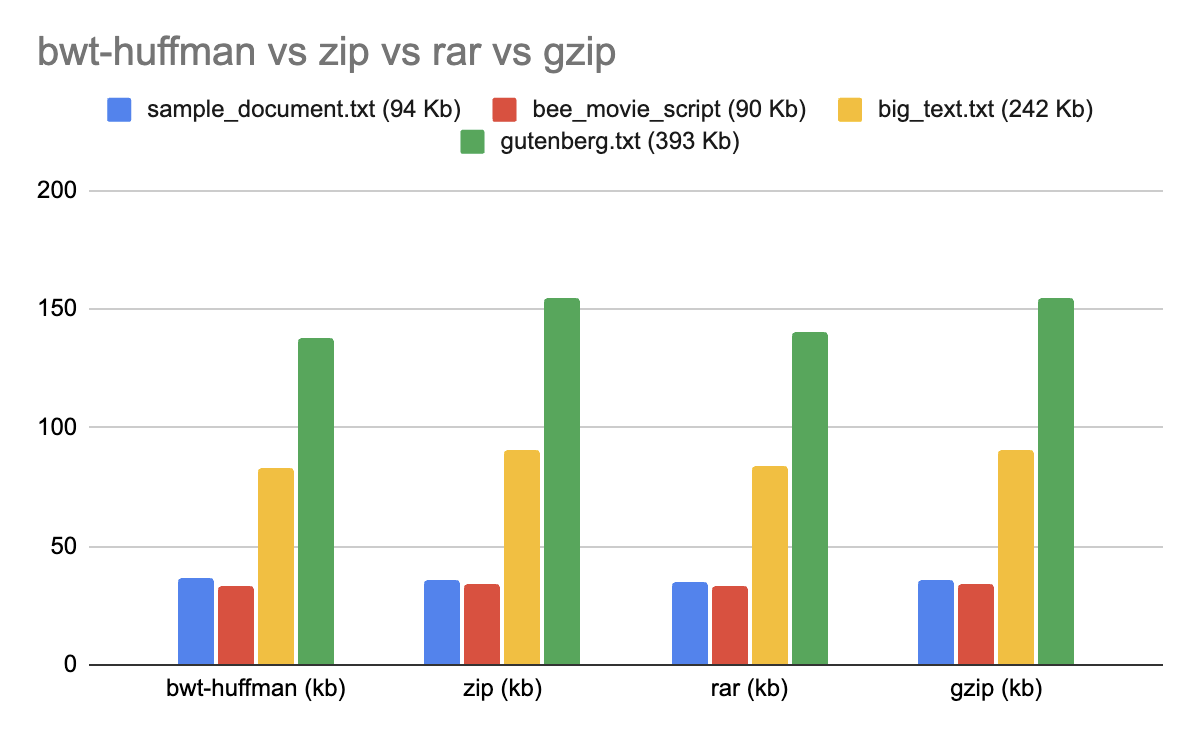
\includegraphics[scale=.5]{./images/chart1.png}
\end{center}


Our implementation is roughly the same size as zip and gzip with the exception of larger files.
At smaller and medium files like 90, 94, 242 kb, and 393 our implementation is roughly the same size
as all the other compression software. However, at larger files like 2,600 kb, our implementation without bwt and mtf algorithms,
is significantly larger than the other compression software. This is most evedent in the office\_hours.bmp file
where our implementation is 6.5 times larger than zip and gzip and almost 9 times larger than rar. 
We then also calculated the compression ratio with the given data. We do this by dividing the size of the original file by the size of the compressed file.

\begin{table}[h]
    \resizebox{\textwidth}{!}{%
    \begin{tabular}{|l|r|r|r|r|}
    \hline
    Ratio                                                & \multicolumn{1}{l|}{bwt-huffman} & \multicolumn{1}{l|}{zip} & \multicolumn{1}{l|}{rar} & \multicolumn{1}{l|}{gzip} \\ \hline
    \cellcolor[HTML]{FFFFFF}sample\_document.txt (94 Kb) & 2.76                             & 2.61                     & 2.69                     & 2.61                      \\ \hline
    bee\_movie\_script (90 Kb)                           & 2.73                             & 2.65                     & 2.73                     & 2.65                      \\ \hline
    big\_text.txt (242 Kb)                               & 2.92                             & 2.66                     & 2.88                     & 2.66                      \\ \hline
    office\_hours.bmp (2600 Kb)                          & 6.58                             & 43.33                    & 59.09                    & 43.33                     \\ \hline
    gutenberg.txt (393 Kb)                               & 2.85                             & 2.54                     & 2.81                     & 2.54                      \\ \hline
    \end{tabular}%
    }
    \caption{Compression Ratio}
\end{table}

The ratios also support our findings along with showing that our implementation is roughly the same ratios for smaller and medium files.
We also compared the time it took to compress the files. 
We mainly tested the time difference between our implementation with bwt and without bwt.
All other compression software were all almost instantanious or just .01 seconds.
\begin{table}[h]
    \resizebox{\textwidth}{!}{%
    \begin{tabular}{|l|r|r|}
    \hline
                                                         & \multicolumn{1}{l|}{With BWT (s)}   & \multicolumn{1}{l|}{Without BWT (s)} \\ \hline
    \cellcolor[HTML]{FFFFFF}sample\_document.txt (94 Kb) & 0.21                                & 0.05                                 \\ \hline
    bee\_movie\_script (90 Kb)                           & 0.22                                & 0.04                                 \\ \hline
    big\_text.txt (242 Kb)                               & 0.56                                & 0.07                                 \\ \hline
    gutenberg.txt (393 Kb)                               & 0.88                                & 0.09                                 \\ \hline
    office\_hours.bmp (2600 Kb)                          & \multicolumn{1}{l|}{Never finishes} & 0.29                                 \\ \hline
    \end{tabular}%
    }
    \caption{Compression Time}
\end{table}

\begin{center}
    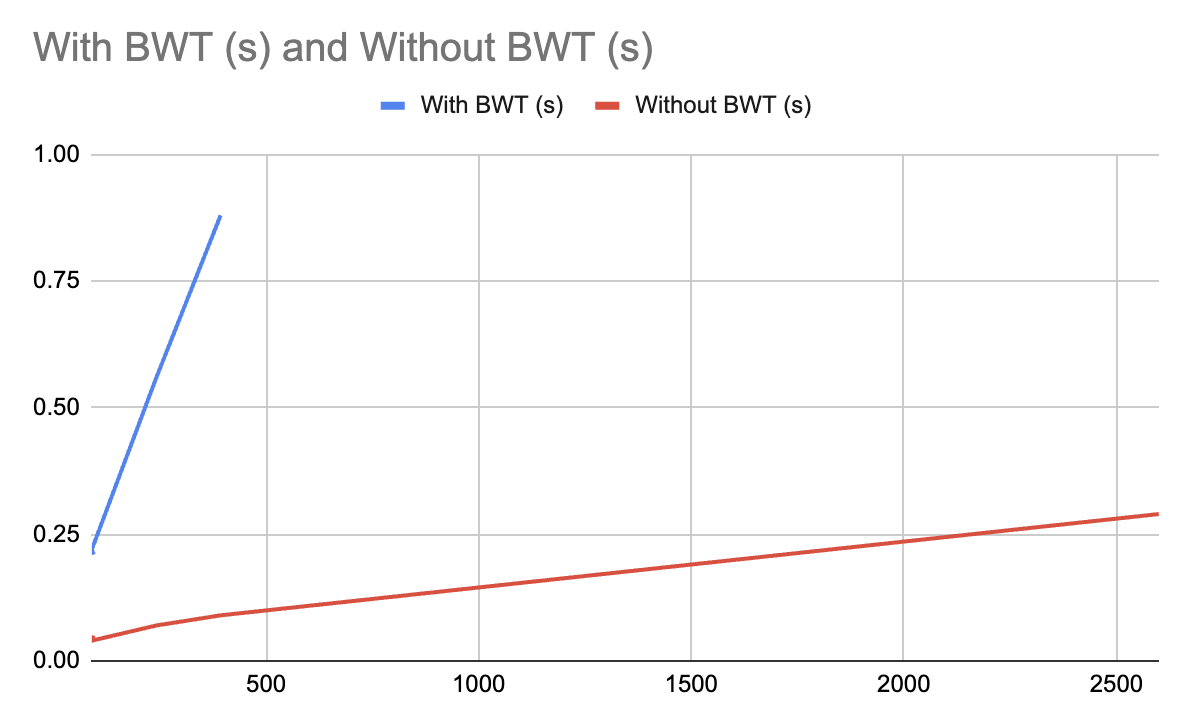
\includegraphics[scale=.5]{images/time.png}
\end{center}

We can see that our implementation with bwt is significantly slower than without bwt.
This is most evident in the office\_hours.bmp file where our implementation with bwt never finishes.
Having to run bwt almost exponentially increases the time it takes to compress the file.
While without bwt it linealy increases the time it takes to compress the file.
This makes sense as bwt is a whole other algorithm that has to be run before encoding which also checks through the entire file.
Though it is slower to compress, we can now check how the compression and its ratio changes with and without bwt.

\begin{table}[h]
    \resizebox{\textwidth}{!}{%
    \begin{tabular}{|l|r|r|}
    \hline
    Compression                                          & \multicolumn{1}{l|}{With BWT (kb)}  & \multicolumn{1}{l|}{Without BWT (kb)} \\ \hline
    \cellcolor[HTML]{FFFFFF}sample\_document.txt (94 Kb) & 34                                  & 51                                    \\ \hline
    bee\_movie\_script (90 Kb)                           & 33                                  & 55                                    \\ \hline
    big\_text.txt (242 Kb)                               & 83                                  & 141                                   \\ \hline
    gutenberg.txt (393 Kb)                               & 138                                 & 226                                   \\ \hline
    office\_hours.bmp (2600 Kb)                          & \multicolumn{1}{l|}{Never finishes} & 395                                   \\ \hline
    \end{tabular}%
    }
    \caption{Compression Size With and Without BWT}
\end{table}

After running with and without bwt, we can see that the compression size is significantly larger without bwt.
This shows now that by sacrificing time, we can get a much better compression.
This shows the importance of bwt as it can significantly reduce the size of the file.
This makes sense as bwt and mtf can arrange the strings in a way where the same strings can be grouped together, making it easier to compress.
The time it takes also makes sense as it is running through the entire file to grab all the strings.

\begin{table}[h]
    \resizebox{\textwidth}{!}{%
    \begin{tabular}{|l|r|r|}
    \hline
    Ratio                                                & \multicolumn{1}{l|}{With BWT (kb)}  & \multicolumn{1}{l|}{Without BWT (kb)} \\ \hline
    \cellcolor[HTML]{FFFFFF}sample\_document.txt (94 Kb) & 2.76                                & 1.84                                  \\ \hline
    bee\_movie\_script (90 Kb)                           & 2.73                                & 1.64                                  \\ \hline
    big\_text.txt (242 Kb)                               & 2.92                                & 1.72                                  \\ \hline
    gutenberg.txt (393 Kb)                               & 2.85                                & 1.74                                  \\ \hline
    office\_hours.bmp (2600 Kb)                          & \multicolumn{1}{l|}{Never finishes} & 6.58                                  \\ \hline
    \end{tabular}%
    }
    \caption{Compression Ratio With and Without BWT}
\end{table}

The ratios also show that the compression ratio is much better with bwt. 
Having bwt is very important in compressing, however for larger files like the bit map,
it would take too long to compress therefore it would be better to compress it without bwt.
The decompression time is also changed with and without bwt.

\begin{table}[h]
    \resizebox{\textwidth}{!}{%
    \begin{tabular}{|l|r|r|}
    \hline
    Decompression Time                                   & \multicolumn{1}{l|}{With BWT (s)}   & \multicolumn{1}{l|}{Without BWT (s)} \\ \hline
    \cellcolor[HTML]{FFFFFF}sample\_document.txt (94 Kb) & 0.09                                & 0.07                                 \\ \hline
    bee\_movie\_script (90 Kb)                           & 0.08                                & 0.08                                 \\ \hline
    big\_text.txt (242 Kb)                               & 0.21                                & 0.14                                 \\ \hline
    gutenberg.txt (393 Kb)                               & 0.36                                & 0.21                                 \\ \hline
    office\_hours.bmp (2600 Kb)                          & \multicolumn{1}{l|}{Never finishes} & 0.31                                 \\ \hline
    \end{tabular}%
    }
    \caption{Decompression Time With and Without BWT}
\end{table}

We can see that the decompression time is much faster without bwt.
This is again contributed to the fact that having to translate the bwt with the inverse bwt takes more time.

\section*{Analysis}

In this assignment we implemented the basis of a bzip2 compression.
We did this by implementing the Huffman encoding algorithm, the Burrows-Wheeler transform, and move-to-front encoding.
We then used these algorithms to compress and decompress a file.
In the benchmarking section, we tested our implementation on several files and compared it to several other compression software.
We compared the compression ratio in table 2 which shows that our implementation 
does very well with smaller and medium files but does not do as well with larger files.
This is because the larger files take too long to compress using bwt and mtf, therefore we 
could only test it without those algorithms. 
The ratio for our implementation is around 2 to 3 from the original file size.
If we were to test it with bwt and mtf, it would
most likely have similar compression ratios to the other compression software.
Overall the compression ratio of our implementation with bwt and mtf is around the same or slightly better than the other compression software.
When we remove bwt and mtf, our implementation does not do as well as the other compression software.
As shown in tables 3, 4, and 5, by removing bwt and mtf, the compression ratio is much worse but much faster.
This is because bwt and mtf are very important in compressing files as they can group similar strings together.
By grouping them together, there are less unique strings to encode which makes it easier to compress.
By grouping them and encoding less unique strings, the compression ratio would then be much better as there are strings to encode, making a smaller file.
The compression ratio without bwt and mtf is around 1.5 to 2 from the original file size which is much worse than the other compression software and our implementation with bwt and mtf.
The time it takes to compress and decompress is also shown in tables 3 and 6 which shows how much faster it is without bwt and mtf.
This is because bwt and mtf take a lot of time to go through the entire file order the strings.
This is why for larger files like the bit map, it is better to compress it without bwt and mtf as going through the entire file would take too long.
Overall, our implementation does very well with smaller and medium files but does not do as well with large files mainly due to the time it takes to compress.

\end{document}